\documentclass[conference]{IEEEtran}
\IEEEoverridecommandlockouts
% The preceding line is only needed to identify funding in the first footnote. If that is unneeded, please comment it out.
\usepackage{cite}
\usepackage{amsmath,amssymb,amsfonts}
\usepackage{algorithmic}
\usepackage{graphicx}
\usepackage{textcomp}
\usepackage{xcolor}
\usepackage{tabularx}
\usepackage{enumitem}
\usepackage{hyperref}
\usepackage[normalem]{ulem}
\useunder{\uline}{\ul}{}

\title{Energy Waste of Docker Smells}

\author{
    \IEEEauthorblockN{Alexander Zwisler}
    \IEEEauthorblockA{
        \textit{Faculty of Mathematics and Computer Science} \\
        \textit{University of Leipzig} \\
        az11kyho@sudserv.uni-leipzig.de
    }
}

\begin{document}

\maketitle
\begin{abstract}
Docker containers are widely used in modern software development, simplifying development, building, and deployment of applications. However, inefficiencies in the creation of Docker containers, so-called \textit{Docker Smells}, arise from developers creating Dockerfiles which contain a suboptimal set of instructions that lead to bloated and inefficient deployments. With growing interest in energy efficient deployments, especially in data centers, the impact of these Docker Smells on energy consumption is worth investigating. This paper aims to explore the impact Docker Smells have on the runtime energy consumption of docker containers. Using real world applications packaged using docker, we run a series of tests, measuring energy consumption with Scaphandre, to provide insight into the impact of docker smells on runtime energy consumption. We conclude that, even though fixing docker smells has a beneficial effect throughout the whole lifecycle of a docker image in terms of energy consumption, the effect on the energy consumption during runtime is negligible.
\end{abstract}

\begin{IEEEkeywords}
Docker, Docker smells, energy consumption, performance, containerization
\end{IEEEkeywords}
\section{Introduction}
In recent years, technologies for containerization have become the standard for development and deployment in modern software development. Docker is one of the most widely adopted containerization tools that provides a lightweight and efficient way for developers to package applications and their dependencies into an isolated environment known as a container \cite{merkel2014docker}. This containerization of the applications significantly reduces the complexity and overhead of running software systems on servers and development machines.

Despite the many advantages Docker brings, it comes with its own problems. One such problem is the usage of suboptimal practices or antipatterns in a Dockerfile, which is used to create the images to run docker containers. These so-called "Docker smells" \cite{durieuxEmpericalStudy} can result in bloated images, longer build times and inefficient use of resources. All of which might ultimately translate into higher energy consumption, a critical concern given the growing emphasis on sustainability in computing \cite{baliga2011green}.

Energy consumption in data centers has been a topic of research for a while now. Studies have shown that data centers account for a significant portion of global electricity usage, making software optimization to reduce energy consumption an interesting topic \cite{koomey2011growth}. In the realm of Docker, the relationship between Docker smells and energy consumption is not very well understood. Previous research has primarily focused on the impact of Docker smells on image size \cite{durieuxEmpericalStudy}, but how these smells might influence the energy consumption of containerized applications remains largely unknown.

Docker smells such as redundant layers, excessive use of the \texttt{RUN} instruction or improper ordering of commands can lead to bloated images that consume more disk space and memory \cite{cito2017empirical}. These inefficient practices not only increase the build time, but also the time and computational resources required for running given containers. Which in turn can lead to higher energy consumption. The larger the image size, the more data must be transferred over the network and stored, which further increases total energy consumption.

Moreover, the energy efficiency of containerized applications is influenced by the underlying infrastructure. Research indicates that the power consumption of containerized environments can vary significantly based on the hardware and host system configuration \cite{morabito2017power}. Tools such as Scaphandre\cite{scaphandre} have been developed to measure the energy usage in real-time, providing valuable insights into how different practices and configurations impact energy consumption \cite{mehulMonitoringEnergy}.

This paper aims to fill the existing research gap of the influence Docker Smells have on energy consumption by investigating the impact of Docker smells on energy consumption. We will conduct a series of experiments using real-world Docker images, measuring their energy usage with Docker Smells present and without the Docker Smells present. We aim to answer the question if and how Docker Smells impact the energy consumption during runtime.


\section{Related Work}

This section reviews the existing literature on Docker smells, their impact on Docker image size, and energy measurement techniques in containerized environments.

\subsection{Docker Smells}

\begin{table*}[h]
    \renewcommand{\arraystretch}{1.2}
    \caption{Analyzed docker smells}
    \label{tbl:smells}
    \begin{tabularx}{\linewidth}{l|X}
    \textbf{Docker Smell} & \textbf{Description} \\ \hline
    \texttt{curlUseFlagL} & The `-L` option in `curl` stands for "follow redirects." When used, curl will follow any redirects encountered when making an HTTP request. Useful for downloading files from URLs that may redirect. \\
    \texttt{npmCacheCleanAfterInstall} & Running `npm cache clean` after `npm install` can reduce image size and ensure the latest version of packages are installed. \\
    \texttt{apkAddUseNoCache} & Using the `--no-cache` flag with `apk add` can prevent issues from outdated packages and ensure the latest version is installed, though it may increase build times. \\
    \texttt{curlUseFlagF} & Using `curl -f` helps prevent build failures if the HTTP request returns an error code >= 400. \\
    \texttt{pipUseNoCacheDir} & Using the `--no-cache-dir` flag with `pip` disables the package cache, ensuring the latest version of a package and its dependencies are installed. \\
    \texttt{aptGetInstallUseNoRec} & Using the `--no-install-recommends` flag with `apt-get install` saves layer space, improves build times, reduces image size and attack surface, and prevents hidden dependencies. \\
    \texttt{aptGetUpdatePrecedesInstall} & Running `apt-get update` and `apt-get install` in a single layer improves efficiency, reliability, and readability. \\
    \texttt{ruleMoreThanOneInstall} & All `apt-get install` commands should be grouped into one. \\
    \texttt{yarnCacheCleanAfterInstall} & `yarn` keeps a local cache of downloaded packages, increasing image size. Clear it by executing `yarn cache clean`. \\
    \texttt{DL3002} & Switching to the root USER opens security risks. Mitigate by switching back to a non-privileged user after necessary root commands. \\
    \texttt{DL3004} & Do not use `sudo` as it leads to unpredictable behavior. Use a tool like `gosu` to enforce root. \\
    \texttt{DL3020} & Use `COPY` instead of `ADD` for files and folders. \\
    \texttt{DL3027} & `apt` is discouraged by Linux distributions for unattended use due to interface changes between versions. Use the more stable `apt-get` and `apt-cache`. \\
\end{tabularx}
\end{table*}

Docker smells refer to anti-patterns and suboptimal practices in Dockerfile creation. Examples of Docker smells can be found in table \ref{tbl:smells}. These smells can lead to various inefficiencies, such as increased image size and longer build times. Several studies have investigated Docker smells and their implications:

\subsubsection{Definition and Identification of Docker Smells}
Docker smells have been identified and categorized in several studies. Duriex et al. \cite{durieuxEmpericalStudy} conducted an empirical study on Dockerfile smells, identifying common smells such as Use of ADD instead of COPY, Installation of unnecessary packages, and Multiple commands in a single RUN instruction. Their study highlights the prevalence of these smells in open-source projects and their impact on maintainability, build efficiency, security and network transfer volume. The study found, that by fixing these inefficiencies in their real world dataset an estimated 40.45 TB a week of data transfer can be avoided when downloading docker images from DockerHub.

\subsection{Parfum: Detection and Automatic Repair of Dockerfile Smells}

Parfum is a tool designed to automatically detect and repair Dockerfile smells. Parfum leverages the Dinghy tool to parse Dockerfiles into an Abstract Syntax Tree (AST), which facilitates easy modification while preserving the original formatting of the files \cite{durieux2023parfumdetectionautomaticrepair}.

The workflow of Parfum consists of several key steps:

\begin{enumerate}
    \item \textbf{Parsing the Dockerfile AST:} Parfum initiates by converting the Dockerfile into an AST representation using Dinghy.
    \item \textbf{Parsing Shell Commands:} Shell commands embedded within the Dockerfile are integrated into the AST, forming a cohesive structure.
    \item \textbf{Enriching the Docker AST:} The AST is further enriched with structural information about command lines and embedded commands.
    \item \textbf{Detecting Docker Smells:} Using a template matching system, Parfum queries the AST to identify known Docker smells. Each smell correlates with specific patterns in the AST.
    \item \textbf{Repairing Docker Smells:} Upon detection of a smell, Parfum repairs it by altering the AST. This involves a template-based approach to generate accurate patches that resemble developer-created patches. The modified AST is then reprinted into a Dockerfile, ensuring only the necessary changes are applied.
\end{enumerate}

The efficacy of Parfum has been validated through extensive evaluation on a large dataset of Dockerfiles, demonstrating high precision and recall in smell detection and successful repair with minimal build failures. The tool has been favorably received by the developer community, with numerous pull requests for smell repairs being accepted and merged into open-source projects \cite{durieux2023parfumdetectionautomaticrepair}.

In summary, Parfum automates the identification and rectification of suboptimal practices in Dockerfiles, assisting developers in maintaining high-quality, efficient Docker images.

\subsection{Prometheus and Grafana}
Prometheus is an open source and monitoring software designed to collect and store metrics as time-series data. It uses a pull based models to scrape metrics from specified applications, or can be used together with the \textit{prometheus-pushgateway} to push the metrics directly into Prometheus. Grafana on the other hand is an open source platform specialized in visualizing and analyzing complex datasets, which integrates seamlessly with Prometheus.

\subsection{Energy Measurement Techniques}

Accurate measurement of energy consumption is crucial for evaluating the efficiency of containerized applications. 

\subsubsection{Power Consumption in Virtualized Environments}
Morabito et al. \cite{morabito2017power} conducted an empirical investigation of power consumption in virtualized environments, comparing the energy usage of containers, virtual machines, and native environments. Their study found that containers consume less power than virtual machines in certain use cases, highlighting the potential energy efficiency benefits of containerization. However, the study also noted that the energy consumption can vary significantly depending on the workload and the specific configurations of the containers and host systems.

\subsubsection{Monitoring Energy Consumption}
Mehul et al. \cite{mehulMonitoringEnergy} show how to monitor docker container energy usage with a hardware based approach. Installing a modified smart power plug between the computer to test and the power grid and using a HLW8032 energy meter sensor to gather current energy consumption readings. This approach proved reliable in identifying and measuring workloads on containerized applications. 

\subsubsection{Energy Efficiency in Data Centers}
The importance of energy efficiency in data centers has been well-documented. Baliga et al. \cite{baliga2011green} discussed the balance of energy consumption in processing, storage, and transport, emphasizing the need for optimizing software to reduce energy usage. Their research highlights that data centers account for a significant portion of global electricity usage, and improving the energy efficiency of containerized applications can contribute to substantial energy savings.

\subsection{Gaps in Existing Research}

While significant progress has been made in understanding Docker smells and measuring energy consumption, gaps remain in the literature. Specifically, the impact of Docker smells on energy consumption has not been thoroughly investigated. Existing studies have focused on the performance implications of Docker smells, such as increased image size and build time \cite{durieuxEmpericalStudy}, but their direct impact on energy usage is still unclear. Furthermore, while tools like Scaphandre provide valuable data on energy consumption, there is a lack of comprehensive studies that link Docker smells to measurable increases in energy usage.

This paper aims to address this gap by investigating how Docker smells influence the energy efficiency of containerized applications. By executing a series of tests with real world applications using docker, we aim to identify the impact of suboptimal practices in the creation of Docker images on energy consumption during the runtime of the container.


\section{Comparison of Energy Measurement Tools: Scaphandre vs. PowerPlug}
To accurately measure the energy consumption of Docker containers, we evaluated two monitoring techniques: Scaphandre and a Smart PowerPlug. This section gives an overview on which technique is more suitable for the given use case.

\subsection{Scaphandre}
Scaphandre is an open-source software agent designed to measure the power consumption of IT hardware, particularly in data centers. It provides detailed insights into the energy usage of containers and virtual machines. It relies on Intel RAPL to estimate the power consumption of individual processes and so-called RAPL Domains. It offers an out-of-the-box solution to provide the usage data to Prometheus and introduces only minimal overhead on the machine running Scaphandre.

\subsection{Power Plug}
The smart power plug is a hardware-based power meter designed to directly measure the energy consumption of the connected device. It can be polled to gather the current consumption data. We developed a script to continuously poll the power plug using the tinytuya\cite{jasonacox/tinytuya} library, which then provides the usage data to Prometheus.
\\
\\
In our initial tests, we compared using Scpahandre against the usage of a hardware based solution. While both solutions were able to accurately measure the power consumption for the most part, the power plug was not able to consistently provide a new reading every 500ms. Also, while a more wholistic picture for the system is given by the data provided by the power plug, this might have an impact on the test execution. During initial stress tests, we could see the power consumption data of the power plug slightly increasing over time, capturing the increased power consumption for cooling the system under high load. See Appendix, Figure \ref{fig:scaph-vs-pp}. Since Scaphandre does not suffer from any of the mentioned problems and provides accurate power reading \cite{kahnRapl}, we decided to use Scaphandre for the experiments. This reduces the amount of other influences in the power consumption data.


% \begin{figure}[htbp]
%     \centering
%     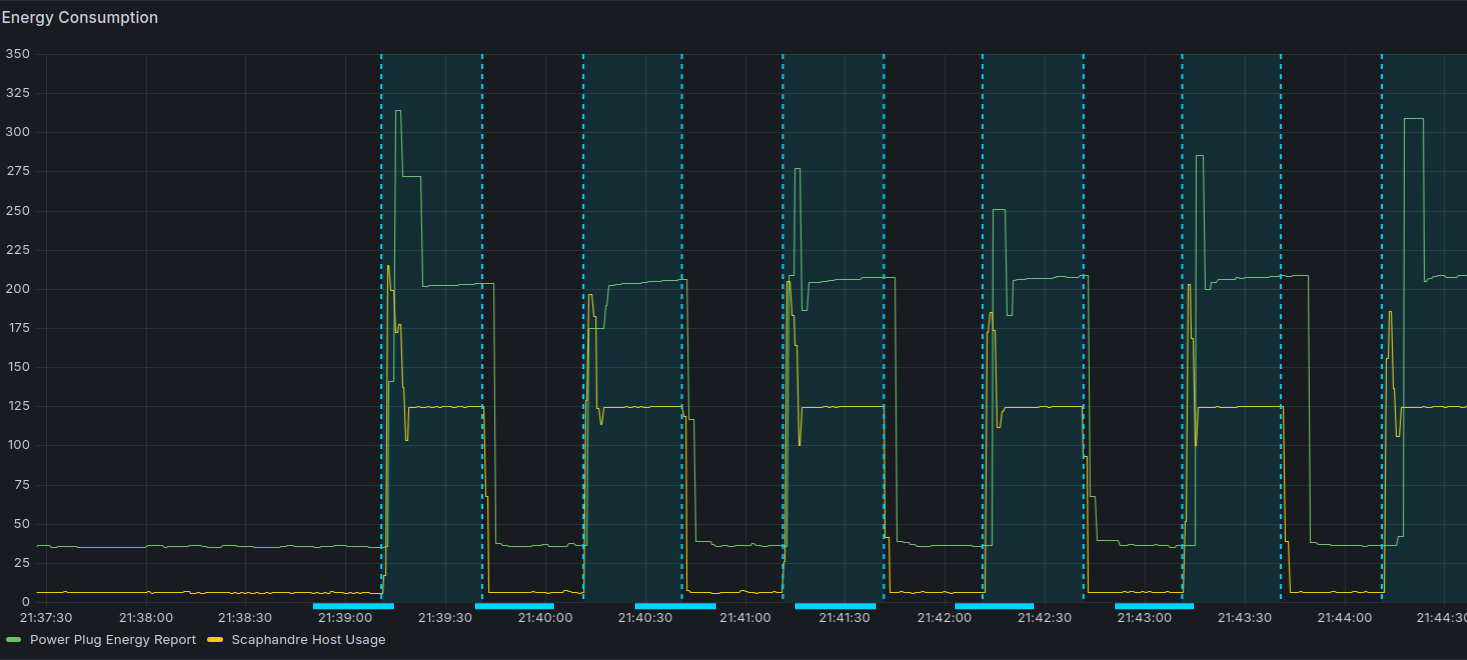
\includegraphics[width=\linewidth]{graphics/scaph_vs_pp.png}
%     \caption{Power Plug vs Scaphandre}
%     \label{fig:docker_smells}
% \end{figure}
\begin{table*}[h]
    \renewcommand{\arraystretch}{1.2}
    \caption{Test repositories}
    \label{tbl:repos}
    \centering
    \begin{tabularx}{\linewidth}{l|l|X}
        Repository & Git hash & Docker smells \\ \hline
        acmesh-official/acme.sh & 0d8a314 & curlUseFlagF, curlUseFlagL \\
        ChatGPTNextWeb/ChatGPT-Next-Web & c359b30 & apkAddUseNoCache, 2x yarnCacheCleanAfterInstall \\
        openai/chatgpt-retrieval-plugin & b28ddce & pipUseNoCacheDir \\
        Chanzhaoyu/chatgpt-web & 574aac2 & 6x npmCacheCleanAfterInstall \\
        gchq/CyberChef & a477f47 & npmCacheCleanAfterInstall \\
        DesignPatternsPHP/DesignPatternsPHP & 41c623c & DL3020, pipUseNoCacheDir \\
        freeCodeCamp/devdocs & 3fab9ef & aptGetInstallUseNoRec \\
        ageitgey/face\_recognition & 2e2dcce & pipUseNoCacheDir, aptGetInstallUseNoRec, aptGetUpdatePrecedesInstall, aptGetInstallThenRemoveAptLists \\
        mattermost/focalboard & 568a5f0 & npmCacheCleanAfterInstall \\
        freqtrade/freqtrade & c227500 & DL3046, pipUseNoCacheDir, 2x aptGetInstallUseNoRec, 2x aptGetInstallThenRemoveAptLists, ruleMoreThanOneInstall \\
        ethereum/go-ethereum & 7cfff30 & DL3020 \\
        Z4nzu/hackingtool & fbffd2e & 2x aptGetInstallUseNoRec, 2x aptGetInstallThenRemoveAptLists, 2x ruleMoreThanOneInstall \\
        derailed/k9s & 626bde1 & curlUseFlagF \\
        parse-community/parse-server & 6bdd87c & 2x npmCacheCleanAfterInstall \\
        jhao104/proxy\_pool & bb16a6f &  2x apkAddUseNoCache \\
        remoteintech/remote-jobs & a87987f & npmCacheCleanAfterInstall \\
        rustdesk/rustdesk & 285e974 & DL3002, DL3004, 2x DL3027, DL3046, curlUseFlagF, curlUseFlagL \\
        coqui-ai/TTS & dbf1a08 & 2x pipUseNoCacheDir, aptGetUpdatePrecedesInstall \\
    \end{tabularx}
 
\end{table*}
\section{Methodology}

\begin{figure}[t]
    \centering
    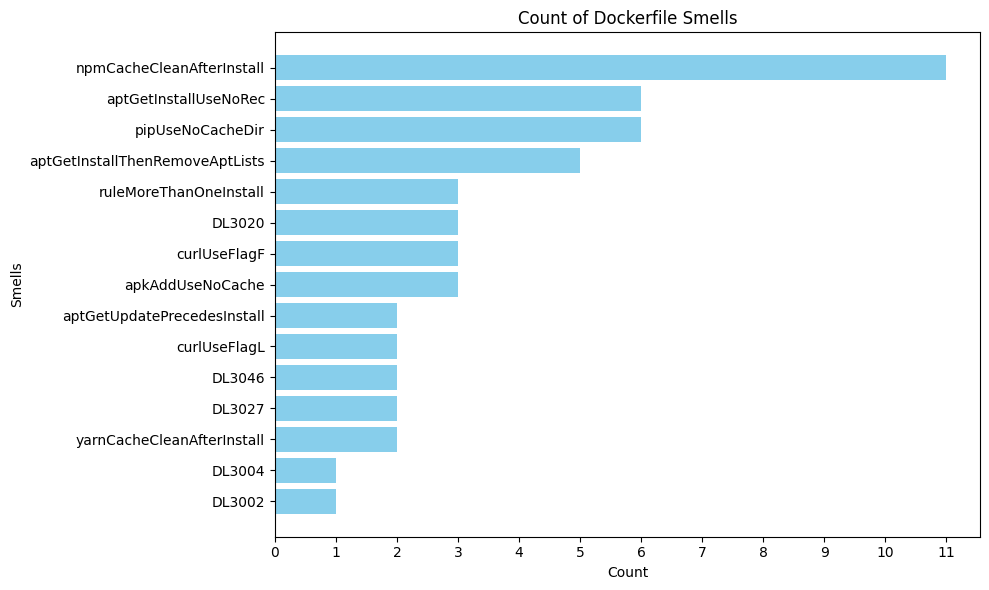
\includegraphics[width=\linewidth]{graphics/docker_smells_in_dataset.png}
    \caption{Test Setup}
    \label{fig:docker_smells}
\end{figure}
\subsection{Dataset}
The dataset for the tests is compiled from publicly accessible GitHub repositories. We selected the most star-rated repositories that contain a Dockerfile and evaluated them using Perfume. If a Dockerfile contained Docker Smells, the corresponding Docker image is created twice: once with the identified problems fixed and once without. This ensures that we can run tests on the given repository. In Table \ref{tbl:repos} the selected Repositories are listed, and the identified Docker Smells are explained in Table \ref{tbl:smells}. Looking at the dataset in figure \ref{fig:docker_smells}, we can see that the most common docker smell are related to package manager caches and increase the image size, where removing these smells can lead to significant savings on image size. As an example, coqui-ai/TTS image size is reduced by close to 3 GB after the removal of the found docker smells.



\subsection{Test Setup}
To evaluate the impact of Docker smells on the energy consumption of applications, we established a controlled experimental setup. The host machine was a newly installed Ubuntu server equipped solely with Docker and Scaphandre. The hardware specifications included a 13th Gen Intel(R) Core(TM) i5-13600K processor and 16 GB of DDR4 RAM, with the swap file size increased to 32 GB to support memory-intensive Docker image builds. A separate monitoring server, configured with Prometheus and Grafana, was used for data collection. It also executed a script which polled the Power Plug consumption data and fed this data into Prometheus. Additionally, a JavaScript application was developed to manage the test execution. In figure \ref{fig:test_setup} an overview of the test setup is displayed, with both the power plug and Scaphandre. 

\begin{figure}[htbp]
    \centering
    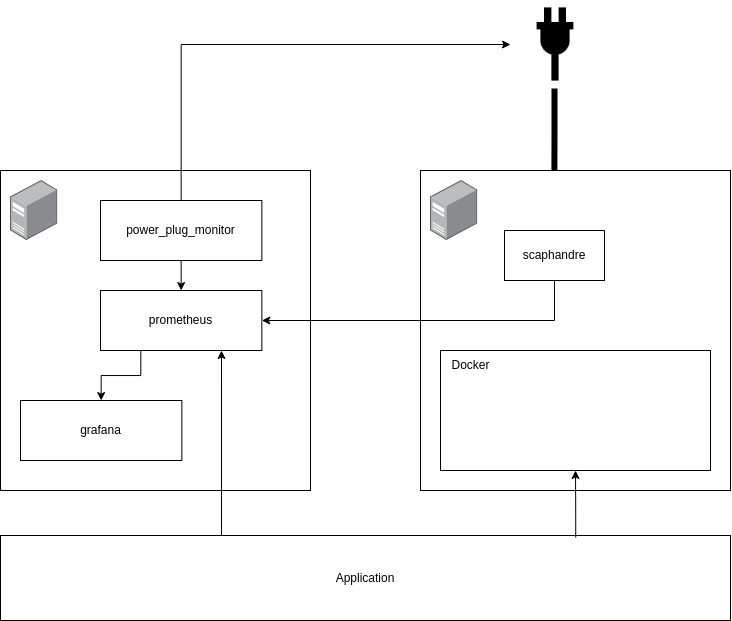
\includegraphics[width=\linewidth]{graphics/setup_double.drawio.png}
    \caption{Test Setup}
    \label{fig:test_setup}
\end{figure}

\subsection{Test execution}
Each repository in the dataset underwent three test iterations to ensure the reliability of the measurements. To exclude the initial power consumption surge associated with container startup, a fixed delay of 30 seconds was implemented before starting the data collection. This delay was determined by initial tests, where startup usually did not take longer than 10 to 15 seconds. We decided to start 10 docker containers from the same image to amplify the impact of the changes. Following the delay, the containers were left idle for 10 minutes, during which energy consumption data was recorded via Scaphandre and Prometheus. For each repository, Docker smells were sequentially removed, and the energy consumption of the resulting images was measured after each modification.

\begin{figure*}[h!]
    \centering
    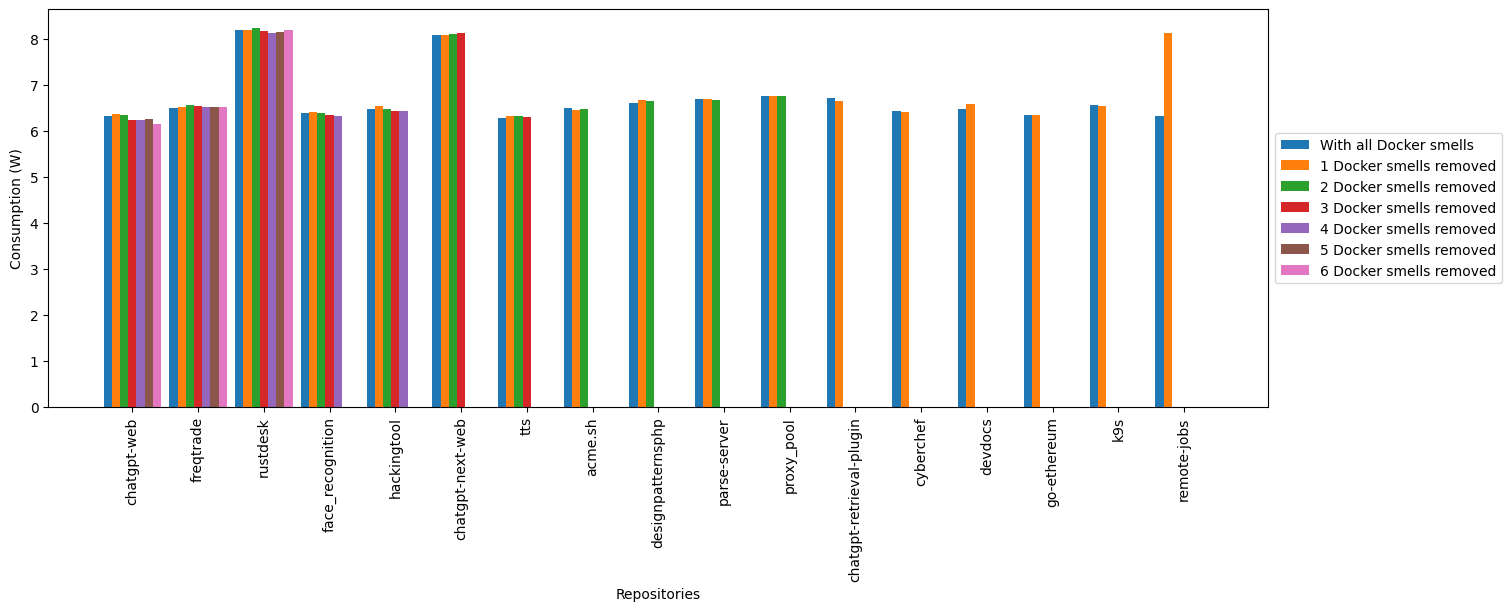
\includegraphics[width=\linewidth]{graphics/repo_avg_consumption_docker_smell.png}
    \caption{Results}
    \textit{Average results of 3 repetitions, grouped by tested repositories with reducing amount of docker smells from left to right}
    \label{fig:docker_smells}
\end{figure*}

\subsection{Energy measurement}
To answer the question, how docker smells impact energy efficiency of docker containers, we need to gather the consumption data during the test execution. We gathered the consumption data in a 500ms interval, to get roughly 1200 data points per performed test. We use three different computers for our tests and verified that the time differences between them are negligible due to synchronization with Linux default NTP server, which manages to get a time difference way below our sampling rate \cite{mills1989accuracy}. With the startup period of 30 seconds and looking only at the average consumption, we do not need millisecond accuracy. The recorded data gets published to Prometheus, which collects the data, until the Application gathers the result at the end of the test. 


\section{Results and Discussion}

\begin{figure}[h]
    \centering
    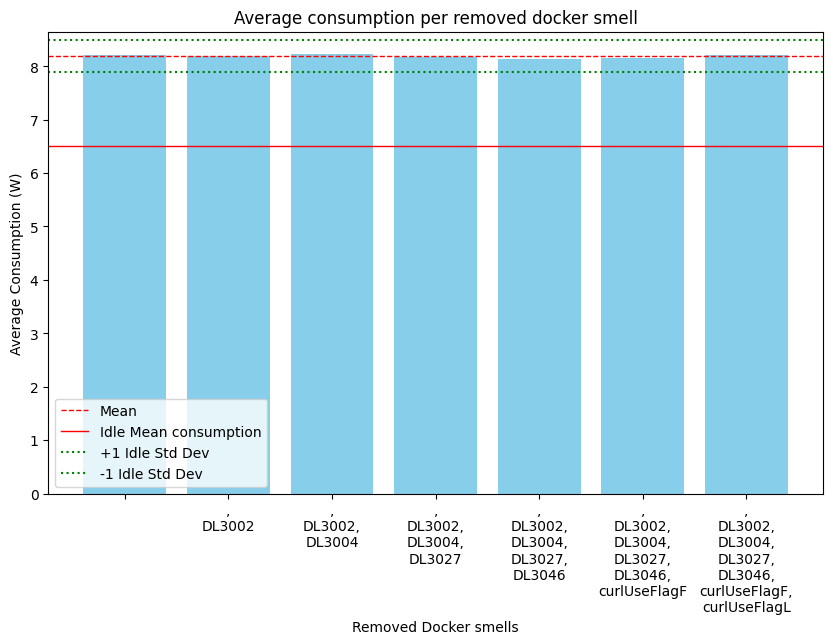
\includegraphics[width=\linewidth]{graphics/rustdesk_widt_std.png}
    \caption{Rustdesk power consumption}
    \textit{Average results of 3 repetitions, with docker smells removed one by one}
    \label{fig:rustdesk}
\end{figure}

The results of the executed tests present a clear picture: common Docker smells, such as uncleared cache folders from package managers, do not lead to higher energy consumption of the running Docker container. Figure \ref{fig:docker_smells} illustrates the results across the 17 repositories tested. Minimal changes in power consumption are observed across different variations of a given Dockerfile, with negligible differences between the variations containing all Docker smells and those containing none. The observed differences in energy consumption can be attributed to the normal fluctuations in system energy consumption, even when the system is idle. We recorded a standard variation of the systems power consumption of \textit{0.3 W} when idle. 

In Figure \ref{fig:rustdesk}, a closer examination of the \textit{rustdesk} repository is presented. The power consumption remains consistent across different variations of the Docker image, staying well within the standard deviation recorded when the system was idle. An exception is noted in the \textit{remote-jobs} repository, where the fixed Dockerfile resulted in a significant increase in power consumption. This spike in energy consumption is likely due to a surge in power consumption during one of the tests, probably caused by an internal Ubuntu system process consuming more power. Figure \ref{fig:remote-jobs-outlier} in the Appendix clearly shows this unusual behavior in the third repetition.

\subsection{Discussion}
The results from our experiments indicate that Docker smells, while increasing image size and build time, do not have a significant impact on the energy consumption of Docker containers. This finding suggests that the inefficiencies introduced by Docker smells are more related to storage and build performance rather than operational energy usage.

One possible explanation for this outcome is that the Docker engine's optimizations and the underlying infrastructure's energy efficiency mitigate the additional resource demands imposed by larger or suboptimally configured images. This is most likely do to the way how docker images manage the layer they consist of. If we look at Figure \ref{fig:docker-layer}, we can see a sketch on how docker layers are stored, layers which are defined in the Dockerfile build the docker image, which by default is stored on the hard drive of the system running the container. On top of the layers of the image, there is a writable layer, which docker uses to allow an application to write to the internal file system. Only this layer is held in RAM. Resulting in the unused data from docker smells to only be contained on the hard drive and never accessed, making their impact on energy consumption negligible.

While the results of the tests seem to indicate that Docker Smells do not have any impact on energy consumption, it is important to note, that all tests were conducted on a single machine, which does not properly reflect server hardware. This makes extrapolating the results to different platforms difficult.

These findings still have practical implications for developers. While it remains essential to follow best practices in Dockerfile creation to optimize build times and reduce image sizes for storage efficiency, the energy consumption of Docker containers during execution appears to be resilient to the presence of Docker smells.


\section{Conclusion}
This study analyzes the impact of Docker smells on energy consumption. Our findings suggest that optimizing Dockerfiles to eliminate these smells does not lead to any improvement on the energy consumption of applications run inside Docker containers during runtime. The way docker is optimized and handles image layers most likely avoids unnecessary resource consumption. Nevertheless, reducing image size and build times will have positive effects on energy consumption thought the whole lifecycle of an application developed and deployed with docker, reducing network traffic and build times. Making it important for developers to reduce the amount of suboptimal construction of docker images. Tools like \textit{Parfume} created by Durieux et al. \cite{durieux2023parfumdetectionautomaticrepair} can help, easily and reliably fix these issues automatically.


\bibliographystyle{IEEEtran}
\bibliography{references}

\newpage

\appendix

\begin{figure}[h]
    \centering
    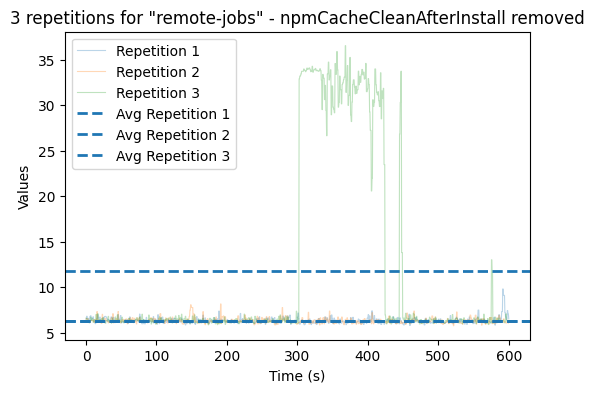
\includegraphics[width=\linewidth]{graphics/remote_jobs_outlier.png}
    \caption{Remote-jobs Repository Outlier on the third repition}
    \textit{}
    \label{fig:remote-jobs-outlier}
\end{figure}

\begin{figure}[h]
    \centering
    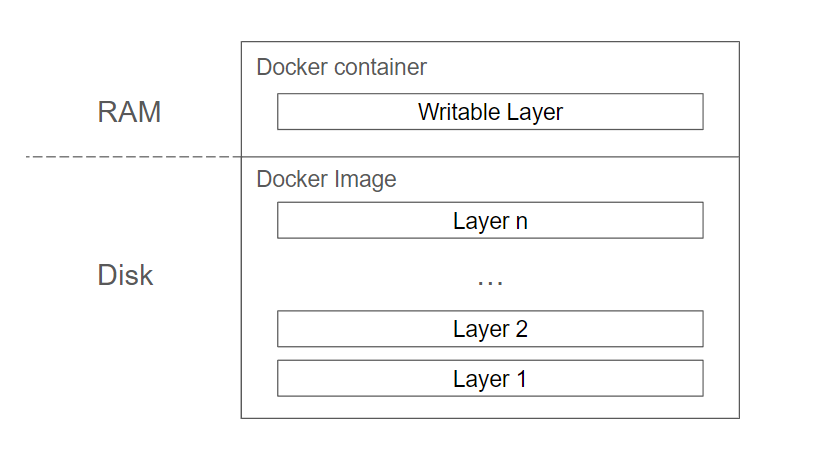
\includegraphics[width=\linewidth]{graphics/docker_layer.png}
    \caption{Docker layer}
    \textit{}
    \label{fig:docker-layer}
\end{figure}


\begin{figure}[h]
    \centering
    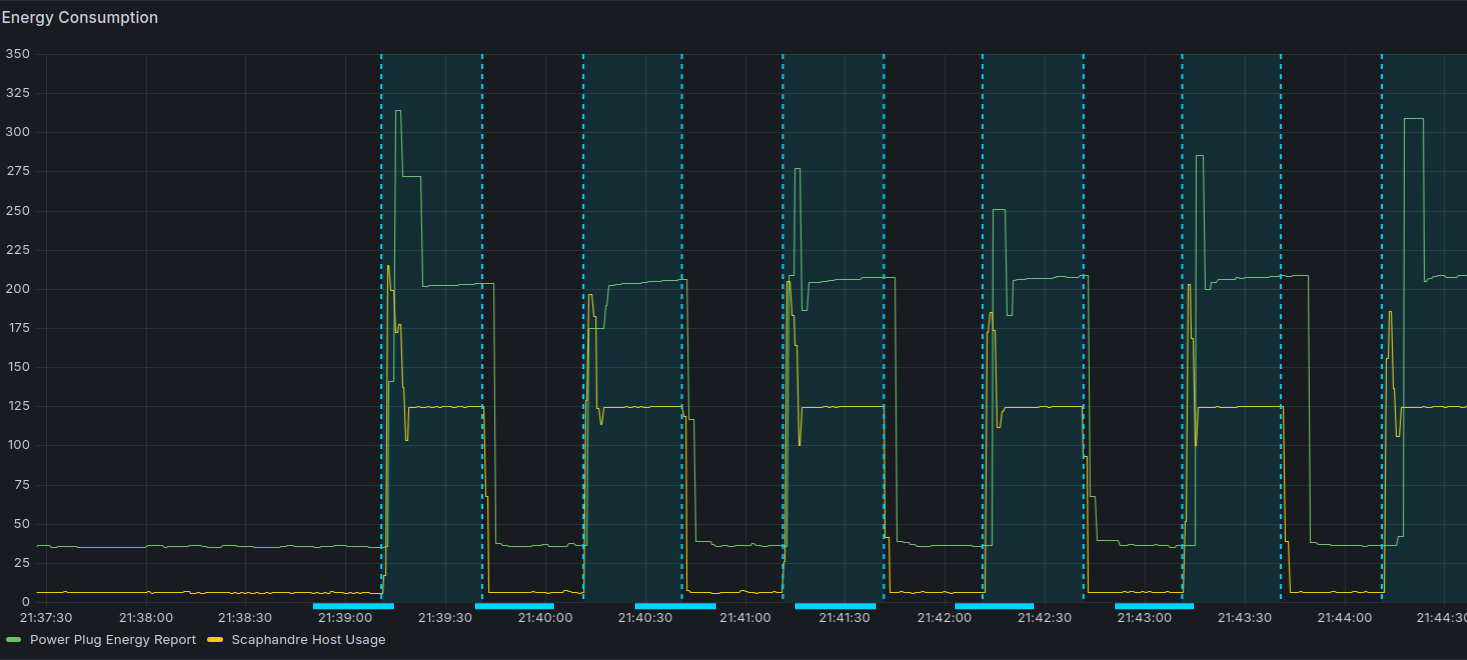
\includegraphics[width=\linewidth]{graphics/scaph_vs_pp.png}
    \caption{Comparison: Power Plug, Scaphandre}
    \textit{}
    \label{fig:scaph-vs-pp}
\end{figure}



\end{document}
